\chapter{Instalar Node.JS y npm}
Desde la versión 0.6.3 de Node.JS, el gestor de paquetes \gls{npm} se instala junto al mencionado entorno de ejecución. En esta sección, se explicarán los pasos a seguir para intalar Node.JS en una máquina con sistema operativo Windows.

\begin{enumerate}
\item Lo primero que debemos hacer es descargar el instalador de Node.JS. Esto lo podemos hacer desde la web oficial de Node.JS (\url{https://nodejs.org/es/download/}). Podremos escoger entre descargarnos la versión \gls{LTS}, que en el momento de escribir este documento se corresponde a la versión 6.9.2, que incluye la versión 3.10.9 de \gls{npm}; o la versión mas actualizada, Node.JS versión 7.2.0 junto con la 3.10.9 de \gls{npm}. Para este manual, hemos escogido la versión mas actual (7.2.0) para Windows x64 en su formato binario (.exe).
\item Una vez descargado el binario, lo ejecutamos apareciéndonos la bienvenida al instalador de node.JS.
\begin{figure}[H]
\centering
  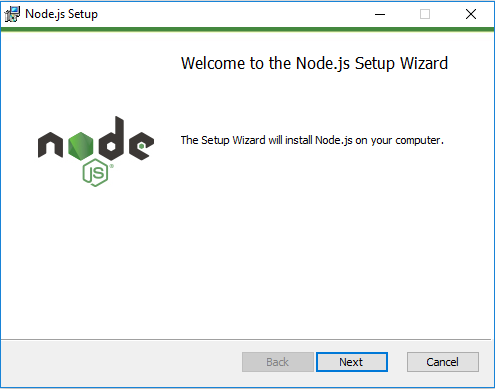
\includegraphics[width=0.8\textwidth]{Figures/anexo/anexoI/nodejs/1}
  \caption{Paso de bienvenida del instalador.}
\end{figure}
\item Pulsamos el botón siguiente, lo que nos llevará a una pantalla con los términos de uso.
\begin{figure}[H]
\centering
  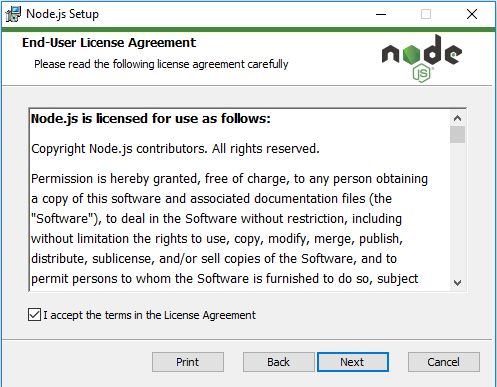
\includegraphics[width=0.8\textwidth]{Figures/anexo/anexoI/nodejs/2}
  \caption{Terminos de uso.}
\end{figure}
\item En el siguiente paso nos permitirá seleccionar la ruta de instalación. Bajo esta ruta se instalarán los scripts ejecutables, por lo que será necesaria recordarla en caso de tener que configurar manualmente las variables de entorno de Windows.
\begin{figure}[H]
\centering
  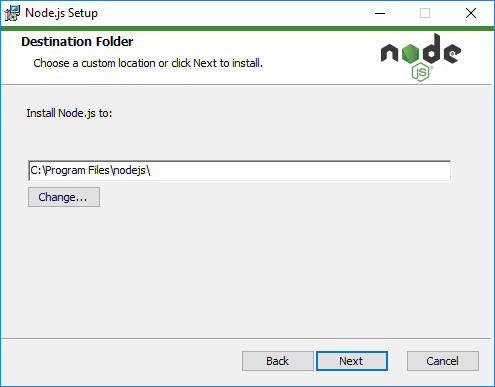
\includegraphics[width=0.8\textwidth]{Figures/anexo/anexoI/nodejs/3}
  \caption{Configuración del directorio de instalación de node.JS.}
\end{figure}
\item Por último nos aparecerá una ventana en la que ya iniciar el proceso de instalación. Será necesario otorgarle permisos de administrador para que pueda realizar la instalación.
\begin{figure}[H]
\centering
  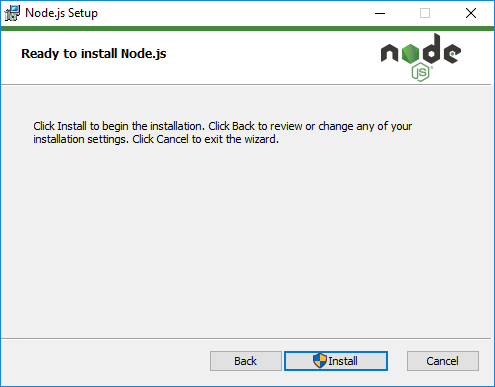
\includegraphics[width=0.8\textwidth]{Figures/anexo/anexoI/nodejs/4}
  \caption{Paso final.}
\end{figure}
\end{enumerate}

Una vez completada la instalación, podremos hacer uso tanto de Node.JS como de npm a través de Windows PowerShell (o de la consola de comandos) o de programas de terceros que hagan uso de estas herramientas.
Para comporbar que la instalación se ha realizado correctamente, desde Windows PowerShell comprobamos la versión de los programas instalados y ejecutamos un pequeño código JavaScript.

\begin{figure}[H]
\centering
  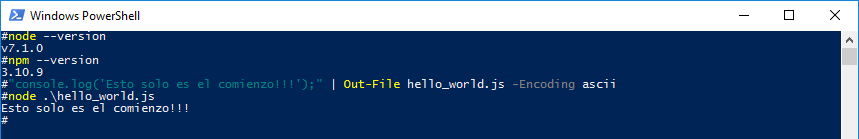
\includegraphics[width=0.8\textwidth]{Figures/anexo/anexoI/nodejs/6}
  \caption{La instalación se ha realizado correctamente.}
\end{figure}

Si el sistema no es capaz de reconocer los comando node o npm, tendremos que chequear que el directorio en el que se realizó la instalación se encuentra configurado en las variables de entorno de Windows. Desde Windows PowerShell se pueden ver estas variables con el siguiente comando:

\begin{lstlisting}[language=bash]
  # Get-ChildItem Env:
\end{lstlisting}
o para ver en más detalle la variable PATH:
\begin{lstlisting}[language=bash]
  # \$Env:PATH
\end{lstlisting}

Si vemos que el directorio de instalación no aparece, tendremos que configurarlo manualmente:
\begin{lstlisting}[language=bash]
  # \$env:Path += ";C:\path\to\node"
\end{lstlisting}
